\documentclass[11pt,border=2pt]{standalone}
\usepackage{tikz}
\usetikzlibrary{decorations.pathmorphing}
\definecolor{linegray}{HTML}{65737E}
\definecolor{measureorange}{HTML}{D97706}
\definecolor{testblue}{HTML}{2563A6}
\begin{document}
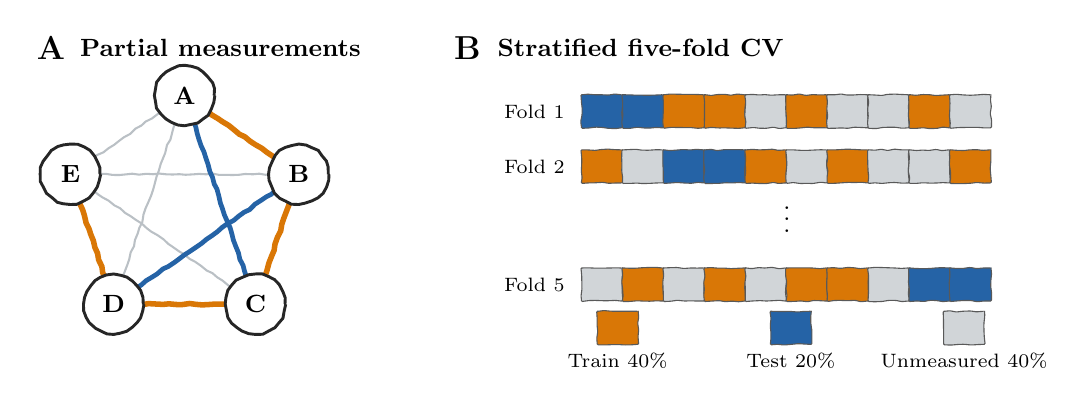
\begin{tikzpicture}[
  sketch/.style={decorate, decoration={random steps, segment length=2.4pt, amplitude=.28pt}},
  candidate/.style={draw=linegray!45, line width=0.75pt, sketch},
  measured/.style={draw=measureorange, line width=2.0pt, sketch},
  held/.style={draw=testblue, line width=1.7pt, sketch},
  taxon/.style={circle, draw=black!85, fill=white, line width=1.05pt, sketch,
    minimum size=7.5mm, inner sep=0pt, font=\small\bfseries},
  paircell/.style={rectangle, rounded corners=.35pt, draw=black!65,
    line width=.4pt, sketch, minimum width=5.2mm,
    minimum height=4.2mm, inner sep=0pt, outer sep=0pt}
]
% Panel A: one distributed-pair example.
\begin{scope}[xshift=0cm]
  \node[anchor=west, font=\large\bfseries] at (0,1.35) {A};
  \node[anchor=west, font=\small\bfseries] at (.55,1.35) {Partial measurements};
  % All 10 possible undirected pairs among five taxa.
  \draw[candidate]
    (2,.75)--(3.45,-.25) (2,.75)--(2.9,-1.9) (2,.75)--(1.1,-1.9)
    (2,.75)--(.55,-.25)
    (3.45,-.25)--(2.9,-1.9) (3.45,-.25)--(1.1,-1.9) (3.45,-.25)--(.55,-.25)
    (2.9,-1.9)--(1.1,-1.9) (2.9,-1.9)--(.55,-.25)
    (1.1,-1.9)--(.55,-.25);
  \draw[held]
    (2,.75)--(2.9,-1.9) (3.45,-.25)--(1.1,-1.9);
  \draw[measured]
    (2,.75)--(3.45,-.25) (3.45,-.25)--(2.9,-1.9)
    (2.9,-1.9)--(1.1,-1.9) (1.1,-1.9)--(.55,-.25);
  \node[taxon] at (2,.75) {A};
  \node[taxon] at (3.45,-.25) {B};
  \node[taxon] at (2.9,-1.9) {C};
  \node[taxon] at (1.1,-1.9) {D};
  \node[taxon] at (.55,-.25) {E};
\end{scope}

% Panel B: five-fold pair evaluation.
\begin{scope}[xshift=5.3cm]
  \node[anchor=west, font=\large\bfseries] at (0,1.35) {B};
  \node[anchor=west, font=\small\bfseries] at (.55,1.35) {Stratified five-fold CV};

  \node[anchor=east, font=\scriptsize] at (1.65,.55) {Fold 1};
  \foreach \i/\c in {0/testblue,1/testblue,2/measureorange,3/measureorange,4/linegray!30,5/measureorange,6/linegray!30,7/linegray!30,8/measureorange,9/linegray!30}
    \node[paircell, fill=\c] at (2.0+.52*\i,.55) {};

  \node[anchor=east, font=\scriptsize] at (1.65,-.15) {Fold 2};
  \foreach \i/\c in {0/measureorange,1/linegray!30,2/testblue,3/testblue,4/measureorange,5/linegray!30,6/measureorange,7/linegray!30,8/linegray!30,9/measureorange}
    \node[paircell, fill=\c] at (2.0+.52*\i,-.15) {};

  \node[font=\small] at (4.35,-.72) {$\vdots$};

  \node[anchor=east, font=\scriptsize] at (1.65,-1.65) {Fold 5};
  \foreach \i/\c in {0/linegray!30,1/measureorange,2/linegray!30,3/measureorange,4/linegray!30,5/measureorange,6/measureorange,7/linegray!30,8/testblue,9/testblue}
    \node[paircell, fill=\c] at (2.0+.52*\i,-1.65) {};

  \node[paircell, fill=measureorange] at (2.2,-2.20) {};
  \node[font=\scriptsize] at (2.2,-2.62) {Train 40\%};
  \node[paircell, fill=testblue] at (4.4,-2.20) {};
  \node[font=\scriptsize] at (4.4,-2.62) {Test 20\%};
  \node[paircell, fill=linegray!30] at (6.6,-2.20) {};
  \node[font=\scriptsize] at (6.6,-2.62) {Unmeasured 40\%};
\end{scope}
\end{tikzpicture}
\end{document}
